\documentclass[letterpaper, 12pt]{article}

\usepackage{caption}
\usepackage[lmargin=1 in, rmargin=1 in, tmargin=1 in, bmargin=1 in]{geometry}
\usepackage{graphicx}
\usepackage{hyperref}
\usepackage{times}
\usepackage{xcolor}

\begin{document}

\setcounter{page}{1}

\begin{center}

\textbf{Data analysis of recordings of slow earthquakes: Tectonic tremor, low frequency earthquakes and slow slip events}

\vspace{1em}

Ariane Ducellier

PhD Dissertation Proposal

October 2019?

\end{center}

\section{Introduction}

The largest earthquakes on Earth occur in subduction zones, where large segments of the boundary between the subducting tectonic plate and the overlying plate can store energy for centuries and then release it in minutes during an earthquake. To better assess seismic hazard, it is thus necessary to improve our understanding of subduction zone processes. Slow slip events are a new feature discovered in the last two decades in many subduction zones thanks to recordings of the displacement of Earth's surface by dense GPS networks. They can last from a few days to several years, and have a relatively short recurrence time (months to years), compared to the recurrence time of regular earthquakes (up to several hundreds of years), allowing scientists to observe and study many complete event cycles, which is typically not possible to explore with traditional earthquake catalogs. 

Moreover, whereas regular earthquakes occur updip of the plate boundary (in the seismogenic / locked zone), slow slip events occur downdip of the plate boundary, in a section adjacent to the locked section of the subduction zone. Interactions between the slow slip zone and the seismogenic zone could potentially trigger large earthquakes. This phenomenon complicates our understanding of subduction zone processes, and should be taken into account when studying the seismic hazard.

As ordinary earthquakes, slow slip events are caused by slip on a fault such as the plate boundary between a tectonic plate subducting under another tectonic plate. However, they take a much longer time (several days to several years) to happen relative to ordinary earthquakes, and the seismic waves they generate are much weaker than the seismic waves generated by ordinary earthquakes, and may not be detectable. A slow slip event on the plate boundary is inferred to happen when there is a reversal of the direction of motion at GPS stations, compared to the secular motion of the surface displacement. Slow slip events have been observed in many subduction zones, such as Cascadia, Nankai (southwest Japan), Alaska, Costa Rica, Mexico, and New Zealand. In many places, tectonic tremor are also observed in relation to slow slip. Tremor is a long (several seconds to many minutes), low amplitude seismic signal, with emergent onsets, and an absence of clear impulsive phases. Tectonic tremor have been explained as a swarm of small, low-frequency earthquakes (LFEs), that is small magnitude earthquakes (M $\sim$ 1) which frequency content (1-10 Hz) is lower than for ordinary earthquakes (up to 20 Hz). In subduction zones such as Nankai and Cascadia, tectonic tremor observations are spatially and temporally correlated with slow slip observations. Due to this correlation, these paired phenomena have been called Episodic Tremor and Slip (ETS). However, this is not always the case. For instance, in northern New Zealand, tremor are more challenging to detect, and seem to be located downdip of the slow slip on the plate boundary.

As ordinary earthquakes, slow slip events are caused by slip on a fault such as the plate boundary between a tectonic plate subducting under another tectonic plate. However, they take a much longer time (several days to several years) to happen relative to ordinary earthquakes, and the seismic waves they generate are much weaker than the seismic waves generated by ordinary earthquakes, and may not be detectable.  A slow slip event on the plate boundary is inferred to happen when there is a reversal of the direction of motion at GPS stations, compared to the secular motion of the surface displacement. Slow slip events have been observed in many subduction zones, such as Cascadia, Nankai (southwest Japan), Alaska, Costa Rica, Mexico, and New Zealand (Beroza and Ide, 2011 ~\cite{BER_2011}; Audet and Kim, 2016 ~\cite{AUD_2016}).

In many places, tectonic tremor are also observed in relation to slow slip. Tremor is a long (several seconds to many minutes), low amplitude seismic signal, with emergent onsets, and an absence of clear impulsive phases. Tectonic tremor have been explained as a swarm of small, low-frequency earthquakes (LFEs ; Shelly \textit{et al.}, 2007 ~\cite{SHE_2007_nature}), that is small magnitude earthquakes (M $\sim$ 1) which frequency content (1-10 Hz) is lower than for ordinary earthquakes (up to 20 Hz). In subduction zones such as Nankai and Cascadia, tectonic tremor observations are spatially and temporally correlated with slow slip observations (Obara, 2002 ~\cite{OBA_2002}; Rogers and Dragert, 2003 ~\cite{ROG_2003}). Due to this correlation, these paired phenomena have been called Episodic Tremor and Slip (ETS). However, this is not always the case. For instance, in northern New Zealand, tremor are more challenging to detect, and seem to be located downdip of the slow slip on the plate boundary.

\section{Proposed PhD Research}

The purpose of my research is to carry out data analyses of recordings of tectonic tremor, low-frequency earthquakes and slow slip events to better understand the mechanism of slow earthquakes. Specifically, I want to be able to better constrain the depth of the source of the tectonic tremor, to detect new low-frequency earthquakes, and to detect smaller and/or longer slow slip events.

\subsection{Depth of the source of the tectonic tremor in the eastern Olympic Peninsula}

\textit{Is the source of the tectonic tremor located on the plate boundary? What is the thickness of the tremor source region?}

\subsubsection*{Motivation}

tremor made of LFEs and LFEs on the plate boundary: tremor should be on the plate boundary but difficult to get depth due to absence of impulsive phases. 
Work by La Rocca et al
origin of tremor qurtz vein (Audet and Burgmann, fagereng etc.). Looks like a much thicker region
Work by Kelin Wang, Michael Bostock?
Determine the depth of the tremor and the thickness of the tremor region

\subsubsection*{Completed work}

Most methods to detect and locate tectonic tremors and LFEs are based on the cross-correlation of seismic signals; either signals at the same station for different events, the same event at different stations, or the same event at a small-aperture array. In this first research project, I am using a slightly modified approach. The available data come from eight small-aperture arrays installed in the eastern part of the Olympic Peninsula, Washington. The aperture of the arrays is about 1 km, and station spacing is a few hundred meters. The arrays are around 5 to 10 km apart from each other. Most of the arrays were installed for nearly a year and were able to record the main August 2010 and August 2011 ETS events. The time and locations (latitude and longitude) of the tremor sources were all computed by Ghosh \textit{et al.} (2012). For each one-minute-long time window where tremor has been detected, I compute the cross-correlation of an horizontal component of the seismogram with the vertical component. Then I compute the average cross-correlation over all the stations of the array. I expect to see better the P-wave on the vertical component, and the S-wave on the horizontal component. As the P- and the S-wave have similar complex source-time functions, I expect to see a peak in the cross-correlation at the time lag between the arrival of the direct P-wave and the arrival of the direct S-wave. Due to the low signal-to-noise ratio of the seismic recordings, this peak is not obvious when I use a single time window. However, when I stack the cross-correlation over all the time windows where the source of the tremor was located at about the same place, I can see a peak appearing in the cross-correlation signal. Using the time lag between the arrival of the P-wave and the arrival of the S-wave for different locations of the tremor and the array, I will be able to determine the depth of the tremor source.

\subsubsection*{Future work}

\subsection{A low-frequency earthquakes catalog for Northern California}

\textit{Do low-frequency earthquakes families behave similarly or differently in Northern California, compared to Washington State and the San Andreas Fault?}

\subsubsection*{Motivation}

The relatively short recurrence of slow slip and tremor events results in a rich history both in space and time and reveals potential patterns.  These event histories have allowed scientists to see complete event cycles, which is typically not possible to explore in traditional earthquake catalogs. However, most of the work on low-frequency earthquakes has been focused on detecting low-frequency earthquakes during periods of high tremor activity, grouping them into families of events, and locating the source of the low-frequency earthquakes families. Longer catalogs (several years) have been established for low-frequency earthquakes families in Mexico (two-year long catalog by Frank \textit{et al.}, 2014 ~\cite{FRA_2014}), the San Andreas Fault (fifteen-year-long catalog by Shelly, 2017 ~\cite{SHE_2017}), and Washington State (five-year-long catalog by Sweet \textit{et al.}, 2019 ~\cite{SWE_2019} and two-year-long catalog by Chestler and Creager, 2017a ~\cite{CHE_2017_JGR} and b ~\cite{CHE_2017_G3}). These studies have shown that low-frequency earthquakes can show a wide range of different behaviors. In northern Washington, Sweet \textit{et al.} (2019) have identified and characterized four different low-frequency earthquakes families that span the width of the transition zone in the Cascadia Subduction Zone beneath western Washington State. They found that the low-frequency earthquakes swarm duration, recurrence interval, and event size decrease systematically with increasing depth. On the San Andreas Fault, Shelly (2017 ~\cite{SHE_2017}) observed a large diversity of recurrence behaviors among the low-frequency earthquakes families, from semicontinuous to highly episodic. Particularly, two families exhibited bimodal recurrence patterns (about 3 and 6 days for the first one, and about 2 and 4 days for the second one). Moreover, he observed an increase in the low-frequency earthquakes event rate after the 2004 Parkfield earthquake. \\

Plourde \textit{et al.} (2015 ~\cite{PLO_2015}) have detected low-frequency earthquakes in Northern California during the April 2008 Episodic Tremor and Slip event using seismic data from the EarthScope Flexible Array Mendocino Experiment (FAME). They used a combination of autodetection methods and visual identification to obtain the initial templates. Then, they recovered higher signal-to-noise low-frequency earthquakes signals using iterative network cross correlation. They found that the low-fequency earthquakes families on the southern Cascadia Subduction Zone were located above the plate boundary, with a large distribution of depths (28-47 km). Three additional families were found on the Maacama and Bucknell Creek faults. On these faults, low-frequency earthquakes tended to occur in bursts, while repeating earthquakes occured as single events or in small groups. Low-frequency earthquakes and regular earthquakes had also different frequency contents. They concluded that dehydration of the mantle and further upward migration of water through the deep crustal fault system could explain the generation of both tremor and regular seismicity on these two faults. \\

I intend to extend the catalog from Plourde \textit{et al.} (2015 ~\cite{PLO_2015}) to the whole two years during which the temporary seismic stations from the FAME experiment were installed, (and possibly to a longer period if the quality of the seismic data allows it) in order to answer two questions:

\paragraph{How is low-frequency earthquakes event rate affected by nearby earthquakes?} I intend to study how low-frequency earthquakes families respond to local perturbations in stress from nearby earthquakes at the Mendocino Triple Junction. The deformation, tectonics, and evolution of southern Cascadia is strongly influenced by the Mendocino Triple Junction, and the Mendocino Triple Junction is one of the most seismically active regions along the Cascadia Subduction Zone. Tremor intensity is affected by regular earthquakes. For instance, tremor in Cascadia is triggered by stresses caused by surface waves from large, distant earthquakes (Rubinstein \textit{et al.}, 2009 ~\cite{RUB_2009}), tremor on the San Andreas is triggered by regional earthquakes (Peng \textit{et al.}, 2009 ~\cite{PEN_2009}; Guilhem \textit{et al.}, 2010 ~\cite{GUI_2010}). Small intraslab earthquakes in Nankai, Japan have also been found to trigger tremor (Han \textit{et al.}, 2014 ~\cite{HAN_2014}). I intend to verify whether a similar pattern can be observed for low-frequency earthquakes.

\paragraph{Are there differences or similarities with the San Andreas Fault, and northern Cascadia?} I intend to study how the behavior of the low-frequency earthquakes families identified by Plourde \textit{et al.} (2015  ~\cite{PLO_2015}) on the two strike-slip faults is similar or differ from the behavior of the low-frequency earthquakes families located on the southern Cascadia Subduction Zone. In particular, I would like to verify whether the low-frequency earthquakes families located on the Maacama and Bucknell Creek fault have a similar behavior to what was observed by Shelly (2017 ~\cite{SHE_2017}) on the San Andreas Fault, and whether the low-frequency earthquakes families located on the southern Cascadia Subduction Zone have a similar behavior to what was observed by Sweet \textit{et al.} (2019 ~\cite{SWE_2019}) on the northern Cascadia Subduction Zone. 

Once I have obtained the new two-year-long catalog of low-frequency earthquakes, I intend to carry out a more thorough statistical analysis of the event occurrence. Long-range dependence is a phenomenon that may arise in the statistical analysis of time series data. It relates to the slow rate of decay of the statistical dependence between two points with increasing time interval between the points. Evidence of long-range dependence has been found in regional earthquakes catalogs (Jimenez \textit{et al.}, 2006) and global earthquakes catalogs (Ogata and Abe, 1991), and in catalogs of mining-induced seismicity (Wglarczyk and Lasocki, 2009). The fractional index $d$ represents how fast the variance in the number of low frequency earthquakes increases with the length of the time window considered. A fractional index such that $0 < d < 0.5$ is characteristic of long-range dependence in the time series. I intend to compute the fractional index for all the families in my new two-year-long catalog, and compare it to the fractional index obtained for catalogs in Mexico (Frank \textit{et al.}, 2014 ~\cite{FRA_2014}), the San Andreas Fault (Shelly, 2017 ~\cite{SHE_2017}), and Washington State (Sweet \textit{et al.}, 2019 ~\cite{SWE_2019} and Chestler and Creager, 2017a ~\cite{CHE_2017_JGR} and b ~\cite{CHE_2017_G3}). \\

Another way of carrying out a statistical analysis of the low-frequency earthquakes occurrence is to use models of seismicity that have been developed to describe, analyze and forecast the probabilities of regular earthquake occurrences. The Epidemic-Type Aftershock Sequence (ETAS) model was introduced by Ogata (1988). It takes account the magnitude frequency distribution law of Gutemberg and Richter (1944) and the Omori-Utsu law of aftershock decay (Omori, 1894; Utsu, 1957), but it allows each event, irrespective of whether it is a small or a big event, to trigger its own offspring. 
ForecastingETAS model for regular earthquake catalogs. Similar for LFE catalogs?

\subsubsection*{Completed work}

We are using a matched-filter algorithm. To detect new low-frequency earthquakes for a given family, we take one hour of seismic data recorded by the permanent stations. Then for each station and each channel (two horizontal and one vertical), we cross-correlate the one-hour long signal with the one-minute long template for the given station and channel. As the signal-to-noise ratio of the seismic data is low, we may not see obvious peaks in the cross-correlation signal. However, if we stack the cross-correlation signals for all the channels and all the stations, we can see peaks appearing. Whenever the value of the average cross-correlation is higher than a threshold (generally eight times the median absolute deviation), we assume that there is a low-frequency earthquake.




  Low-frequency earthquakes are usually grouped into families of events, with all the earthquakes of a given family originating from the same small patch on the plate interface, and recurring more or less episodically in a bursty manner. When enough (a few hundred) low-frequency earthquakes have been identified for a given family, a template waveform can be obtained by stacking all the waveforms corresponding to all the low-frequency earthquakes identified. Once a template is available, additional low-frequency earthquakes can be found by cross-correlating seismic data with the template, and assuming that a low-frequency earthquake is occurring whenever the value of the cross-correlation is higher than a chosen threshold.  The signal-to-noise ratios are low, so low-frequency earthquakes can be best identified by stacking the cross-correlation functions of multiple stations.


We are currently using data from a temporary experiment in Northern California. A hundred seismic stations have been installed between 2007 and 2009. Low-frequency earthquakes have been detected, and templates for 66 families have been obtained by Plourde et al. (2015) using data recorded during a period of high tremor activity in April 2008. We are currently using their templates to extend their catalog to the whole two years during which the temporary seismic stations were installed.

It turns out that these low-frequency earthquakes were also detected by the stations from three permanent seismic networks (Berkeley Digital Seismic Network, Northern California Seismic Network, and Plate Boundary Observatory). These stations have been installed as early as 2001 and are still recording seismic data. We thus have 18 years of data available. The aim of this project is thus to extend our catalog of low-frequency earthquakes from two years to eighteen years.

n a related research project, I analyzed catalogs of LFEs from the Olympic Peninsula, Northern California, Mexico, and the San Andreas Fault. For each family of LFEs, I translated the catalog into a continuous time series defined by number of events per minute. The sample interval is 1 minute. Then, I computed the value of the fractional parameter $d$, which represents how fast the variance in the number of LFEs increases with the length of the time window considered. For most families of the catalogs studied, I found that $0 < d < 0.5$, which is characteristic of long-range dependence in the time series. The only exception is the San Andreas Fault catalog, where the LFE families show a wider range of behaviors, and where only some of the families exhibit evidence for long-range dependence. Long-range dependence may be explained by interactions among several asperities associated with the same LFE family. The statistical characterization of LFE occurrence could provide important constraints on future mechanical models of slow earthquake phenomena.

\subsubsection*{Future work}

\subsection{Detection of slow slip events in New Zealand}

\textit{Can we detect small and / or longer slow slip events in the absence of spatially and temporally correlated tectonic tremor?}

\subsubsection*{Motivation}

As ordinary earthquakes, slow slip events are caused by slip on a fault such as the plate boundary between a tectonic plate subducting under another tectonic plate. However, they take a much longer time (several days to several years) to happen relative to ordinary earthquakes, and the seismic waves they generate are much weaker than the seismic waves generated by ordinary earthquakes, and may not be detectable.  A slow slip event on the plate boundary is inferred to happen when there is a reversal of the direction of motion at GPS stations, compared to the secular motion of the surface displacement. Slow slip events have been observed in many subduction zones, such as Cascadia, Nankai (southwest Japan), Alaska, Costa Rica, Mexico, and New Zealand (Beroza and Ide, 2011 ~\cite{BER_2011}; Audet and Kim, 2016 ~\cite{AUD_2016}). \\

In many places, tectonic tremor are also observed in relation to slow slip. In subduction zones such as Nankai and Cascadia, tectonic tremor observations are spatially and temporally correlated with slow slip observations (Obara, 2002 ~\cite{OBA_2002}; Rogers and Dragert, 2003 ~\cite{ROG_2003}). Due to this correlation, these paired phenomena have been called Episodic Tremor and Slip. However, this is not always the case. For instance, in northern New Zealand, tremor are more challenging to detect, and seem to be located downdip of the slow slip on the plate boundary. \\

New Zealand exhibits a wide range of slow slip behavior, and is therefore an exciting site for research. The tectonics of the North Island of New Zealand is dominated by the westward subduction of the Pacific Plate under the Australian Plate at the Hikurangi Trench. Two types of slow slip events have been observed at the Hikurangi margin. Shallow (10-15 km depth), shorter (1-3 weeks), and usually smaller (Mw 6.3-6.8) slow slip events have been observed every 18-24 months in the northern part of the margin. Deeper (35-60 km depth), longer (12-18 months), and larger (Mw 7.0) slow slip events have been observed every 5 years in the southern part of the margin (Wallace and Beavan, 2010 ~\cite{WAL_2010}; Todd and Schwartz, 2016 ~\cite{TOD_2016}).\\

It used to be thought that there were no tremor associated with slow slip events in northern Hikurangi. Delahaye \textit{et al.} (2009 ~\cite{DEL_2009}) observed an increase in the rate of microseismicity downdip of the 2004 Gisborne slow slip event. More recently however, Kim \textit{et al.} (2011 ~\cite{KIM_2011}) detected a low level of tremor activity that increased during the 2010 Gisborne slow slip event. As was the case for the microearthquakes, the source of the tremor was located downdip of the slow slip patch determined from GPS data. Ide (2012 ~\cite{IDE_2012}) detected tremor downdip of the location of two deep slow slip events observed by Wallace and Eberhart-Phillips (2013 ~\cite{WAL_2013}) in 2006 and 2008. However, contrary to Episodic Tremor and Slip events in Cascadia and Nankai, the tremor activity did not seem to increase during the slow slip events. Todd and Schwartz (2016 ~\cite{TOD_2016}) detected tremor associated with most of the shallow slow slip events between 2010 and 2015, and located downdip of the geodetically inferred slip area. They also detected deeper tremor between 20 and 50 km depth with unclear origin. They hypothesized that these tremor may be related to currently undetected deep long-term slow slip events.\\

In other subduction zones, tremor has been used as a proxy to study slow slip events. For instance, Aguiar \textit{et al.} (2009 ~\cite{AGU_2009}) used the tremor occurrence rate to determine the moment released by short tremor episodes for which no slow slip is detectable in the GPS data. Frank (2016 ~\cite{FRA_2016}) stacked independently the displacement observed on GPS data during time periods when low-frequency earthquakes are detected, and the displacement observed during time periods when no low-frequency earthquake is detected, and succeeded in observing surface deformation previously hidden in GPS noise. However, as there is no clear relationship between tremor and slow slip occurrence in New Zealand, these methods cannot be applied, and we need other methods to be able to better detect and quantify slow slip.\\

Several questions could be explored regarding slow slip in northern New Zealand:

\paragraph{Detecting smaller, currently undetected slow slip events.} This would help us to verify whether the fault weakens with depth. Indeed, it has been observed in Cascadia that, with decreasing depth, there is a gradation from frequent tremor episodes with small spatial and temporal extent, to infrequent tremor episodes with large spatial and temporal extent (Wech and Creager, 2011 ~\cite{WEC_2011}). The same behavior was observed for low-frequency earthquakes with downdip low-frequency earthquakes swarms happening nearly weekly and up-dip families only occurring during the yearly Episodic Tremor and Slip events (Sweet \textit{et al.}, 2019 ~\cite{SWE_2019}). As there is a temporal and spatial correlation between slow slip, tremor and low frequency earthquakes, the same spatial pattern is also expected for the slow slip. However, the limited resolution of geodetic instruments only allows us to observe the largest slow slip events, and many smaller slow slip events may be undetected. It has been hypothesized that stable sliding at depth transfers stress to the base of the Episodic Tremor and Slip zone, initiating frequent tremor and small slow slip. In a self-similar process, stress is then transferred up-dip of the fault, triggering less frequent tremor and larger slow slip, up toward the locked zone. This unobserved up-dip slip could help mediate plate convergence and either lower the slip deficit available for co-seismic slip or shift the downward extent of the megathrust rupture away from urban centers (Wech and Creager, 2011 ~\cite{WEC_2011}). Similarly, smaller slow slip events may exist in New Zealand. However, without a good spatiotemporal correlation with tremor occurrence, they are even harder to detect.

\paragraph{Detecting longer term slow slip events.} Long term slow slip events have been detected in Japan, Mexico, Alaska, and possibly Cascadia. Todd and Schwartz (2016 ~\cite{TOD_2016}) detected deep tremor between 20 and 50 km depth with unclear origin and hypothesized that these tremor may be related to deep long-term slow slip events, but were unable to detect them. Indeed, as a long-term slow slip event releases the same seismic moment at the plate boundary during months (or years) as what is released in a few weeks by a short-term slow slip event, we cannot see a sharp jump in the ground displacement time series, but a slow increase that is harder to detect. 

\paragraph{Better measuring of the vertical displacement at the Earth's surface during slow slip events.} This is necessary to better constrain the depth extent of the slip area at the plate boundary. The up-dip limit of the slow slip area is assumed to be one of the constraints on the down-dip limit of the megathrust earthquake rupture, a variable that is currently being used in Cascadia for seismic hazard studies, and the design of building codes. Constraining the down-dip limit of slow slip is also useful to estimate the area that slips during a slow-motion earthquake, and thus the percentage of the plate convergence that is released by large slow slip episodes. Additionally, the up-dip and down-dip limits of slow slip can be correlated with other geophysical data, such as porosity, temperature, and structure, in an effort to better understand the underlying processes that facilitate aseismic slip. The vertical component of the ground displacement is the most useful in constraining the up-dip and down-dip extent of slip since the sense of motion (uplift versus subsidence) changes for slip at different depths (Szeliga \textit{et al.}, 2008 ~\cite{SZE_2008}). However, the vertical displacement is smaller than the horizontal displacement, and generally hard to resolve.

\subsubsection*{Completed work}

I am using data made publicly available by GeoNet, which is a partnership between the Earthquake Commission of New Zealand, GNS Science, and Land Information New Zealand. Ground deformation data are collected continuously by GeoNet using Global Navigation Satellite System (GNSS) receivers and antennas. Daily time series solutions can be easily obtained from GeoNet's website. The coordinates and their formal uncertainties are extracted during the GLOBK run from the combined daily solution files, and converted to (east, north, up) displacement in millimeters with respect to an a priori position and epoch in the ITRF2008 realisation. The resulting time series have no adjustments made to them, so they may, for example, contain offsets due to earthquakes, offsets due to equipment changes at individual sites, and seasonal (annual and semi-annual) signals due to various causes. \\

I have started to develop a Python library implementing wavelet methods for time series analysis. The Discrete Wavelet Transform (DWT), and its alternative the Maximal Overlap Discrete Wavelet Transform (MODWT), transform a time series $X_t$ into a series of vectors of wavelet coefficients $W_j \left(  j= 1 , ... , J \right)$, where $J$ is the level of the wavelet decomposition (Percival and Walden, 2000 ~\cite{PER_2000}). Each wavelet vector $W_j$ is associated with changes on scale $\tau_j = dt 2^{j - 1}$, where $dt$ is the time step of the time series, and corresponds to the filtering of the original time series with a filter with nominal frequency interval $\lbrack \frac{1}{dt 2^{j + 1}} ; \frac{1}{dt 2^j} \rbrack$. The scaling vector $V_J$ is associated with averages in scale $\lambda_J = dt 2^J$, and corresponds to the filtering of the original time series with a filter with nominal frequency interval $\lbrack 0 ; \frac{1}{dt 2^{J + 1}} \rbrack$. Using the wavelet coefficients, we can compute the $j$th wavelet detail $D_j$ and the $J$th wavelet smooth $S_J$. Together, the details and the smooth define the multiresolution analysis (MRA) of $X$: $X = \sum_{j = 1}^{J} D_j + S_J$. The main advantage of the MODWT over the DWT is that when we circularly shift the time series, the corresponding wavelet vectors, scaling vector, details and smooth are shifted by the same amount. Moreover, the details and the smooth are associated with a zero phase filter, making it easy to meaningfully line up the features of the MRA with the original time series. \\

As an example, I have carried out the MODWT and the MRA for the eastern component of the time series recorded at five stations in the Northern Island of New Zealand (PUKE, ANAU, GISB, MAHI, and CKID). The 6\textsuperscript{th} level detail for each station is plotted in Figure X. It corresponds to changes on scale 64 days, which is about twice the duration of a slow slip event. The grey bars show the time of the transients listed by Todd and Schwartz (2016 ~\cite{TOD_2016}, their Table 1). For station CKID, all the peaks observed in the 6\textsuperscript{th} level detail between 2010 and 2015 correspond to a slow slip event. For stations GISB and MAHI, the main peaks observed in the 6\textsuperscript{th} level detail between 2010 and 2015 correspond to a slow slip event. However, not all slow slip events are associated with peaks in the 6\textsuperscript{th} level detail. It may be because they have a shorter duration (and thus should be seen on a lower level detail), or are too close to each other. Slow slip events are less obvious for stations ANAU and PUKE, maybe because they happen very closely to each other. \\

An important application of the DWT and the MODWT is the estimation of a signal hidden by noise within an observed time series. The main idea is to modify the elements of the wavelet vectors $W_j$, to produce new wavelet vectors $W'_j$ from which an estimate of the signal can be synthesized using the inverse wavelet transform. The wavelet vectors can be transformed using thresholding, scaling, or shrinkage (Percival and Walden, 2000 ~\cite{PER_2000}). As an example, Figure X shows a synthetic time series with slow slip events of durations 20 and 50 days, to which a Gaussian noise has been added, the corresponding denoised signal obtained using thresholding of the wavelet vectors, and the signal obtained with a low-pass filter. Although the signal is barely visible behind the noise in the left-hand panel with duration 20 days and signal-to-noise ratio 1, we can see in the denoised signal that there is a unique ramp-like signal in the data, whereas the low-pass filtered signal shows several ramp-like features. \\

I have applied this denoising method to GPS time series. Figure X shows the denoised time series obtained applying the thresholding method to the eastern and the vertical components of the displacement at GPS station CKID, located in the North Island of New Zealand. The denoising and the low-pass filtering give similar results for the horizontal component, but the denoising highlights different features for the vertical component.

\subsubsection*{Future work}

\paragraph{Detecting smaller, currently undetected slow slip events.} I intend to combine MRA of several channels and several stations, and stack them with some time shift to take into account a possible propagation of the slow slip event along the plate boundary, in order to get a better wavelet signal, and be able to see peaks in the wavelet details currently unseen. Another possibility is to use a matching pursuit algorithm. The idea is to approximate the time series by a small number of basis wavelet vectors (Mallat and Zhang, 1993 ~\cite{MAL_1993}) in order to obtain an adaptive time / frequency decomposition of the time series by using a sum of waveforms whose localizations in time and frequency match those of pertinent structures in the time series (Percival and Walden, 2000 ~\cite{PER_2000}). Regarding this research problem, I expect that the first wavelet basis vectors obtained with the matching pursuit algorithm will correspond to the biggest slow slip events, but that some other wavelet basis vectors that could be associated with smaller events will also appear in the decomposition.

\paragraph{Detecting longer term slow slip events.} I expect that longer term slow slip events could be seen on the wavelet details at larger scale. However, computing these details at larger scale requires having a continuous time series. Currently, there are some missing data in the GPS recordings due to instrumental dysfunction. I intend to replace the missing data points by synthetic data points obtained by a combination of linear or more complex interpolation and random Gaussian noise. To verify whether the method chosen to deal with missing data points could affect the results of the wavelet analysis, I will test the method on the GPS stations where long time series without missing data are available. I will remove one or more existing points, replace them using different interpolation methods, and compare the MRA obtained with the original points and the interpolated points.

\paragraph{Better measuring of the vertical displacement at the Earth's surface during slow slip events.}  I intend to use wavelet-based methods to denoise the time series, by applying thresholding, scaling, or shrinkage of the wavelet coefficients before reconstructing the time series using the inverse wavelet transform. I will test several denoising methods. If one of them improve the accuracy of the measurement of the vertical displacement during a slow slip event, the results may be used to carry out inversions of slow slip events, and obtained the slip history of the fault at depth. 

\newpage
\setcounter{page}{1}

\bibliographystyle{plain}
\bibliography{bibliography}

\newpage
\setcounter{page}{1}

\section*{Figures}

\begin{center}
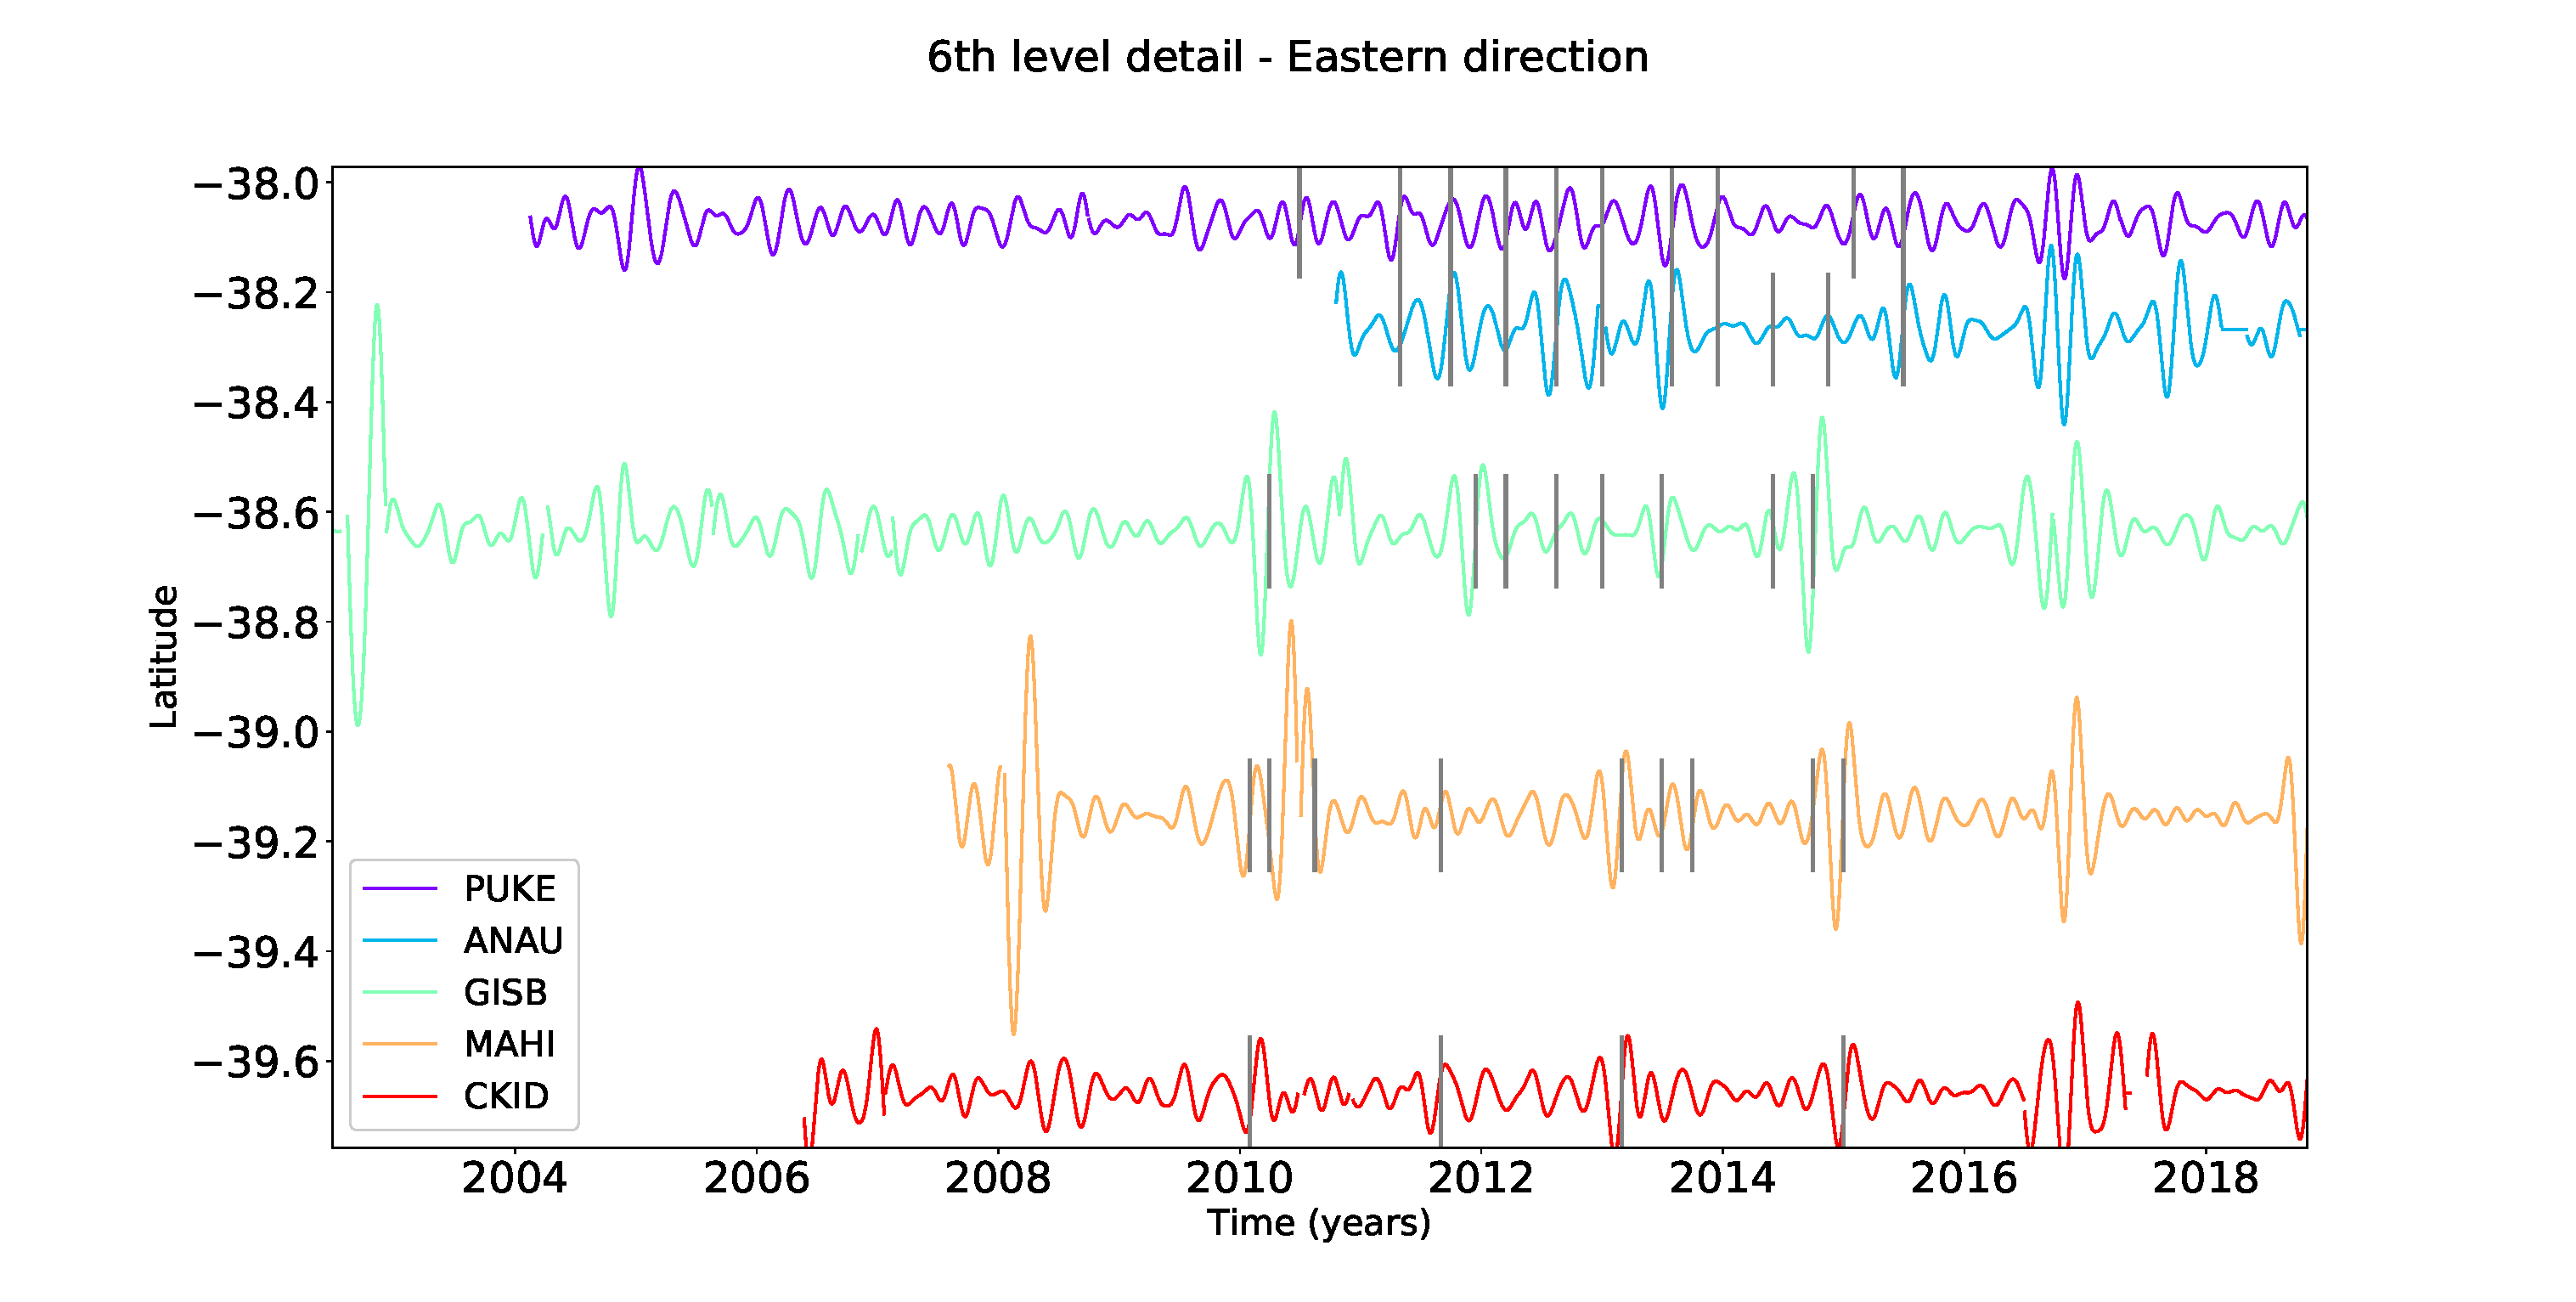
\includegraphics[trim={2.5cm 0.5cm 5cm 0.5cm}, clip, width=400pt]{figures/slowslip_MRA.eps}
\captionsetup{type=figure}
\captionof{figure}{6\textsuperscript{th} level detail of the MRA for the eastern component of the time series recorded at stations PUKE, ANAU, GISB, MAHI, and CKID. The grey bars show the time of the transients listed by Todd and Schwartz (2016 ~\cite{TOD_2016}, their Table 1).}
\end{center}

\begin{center}
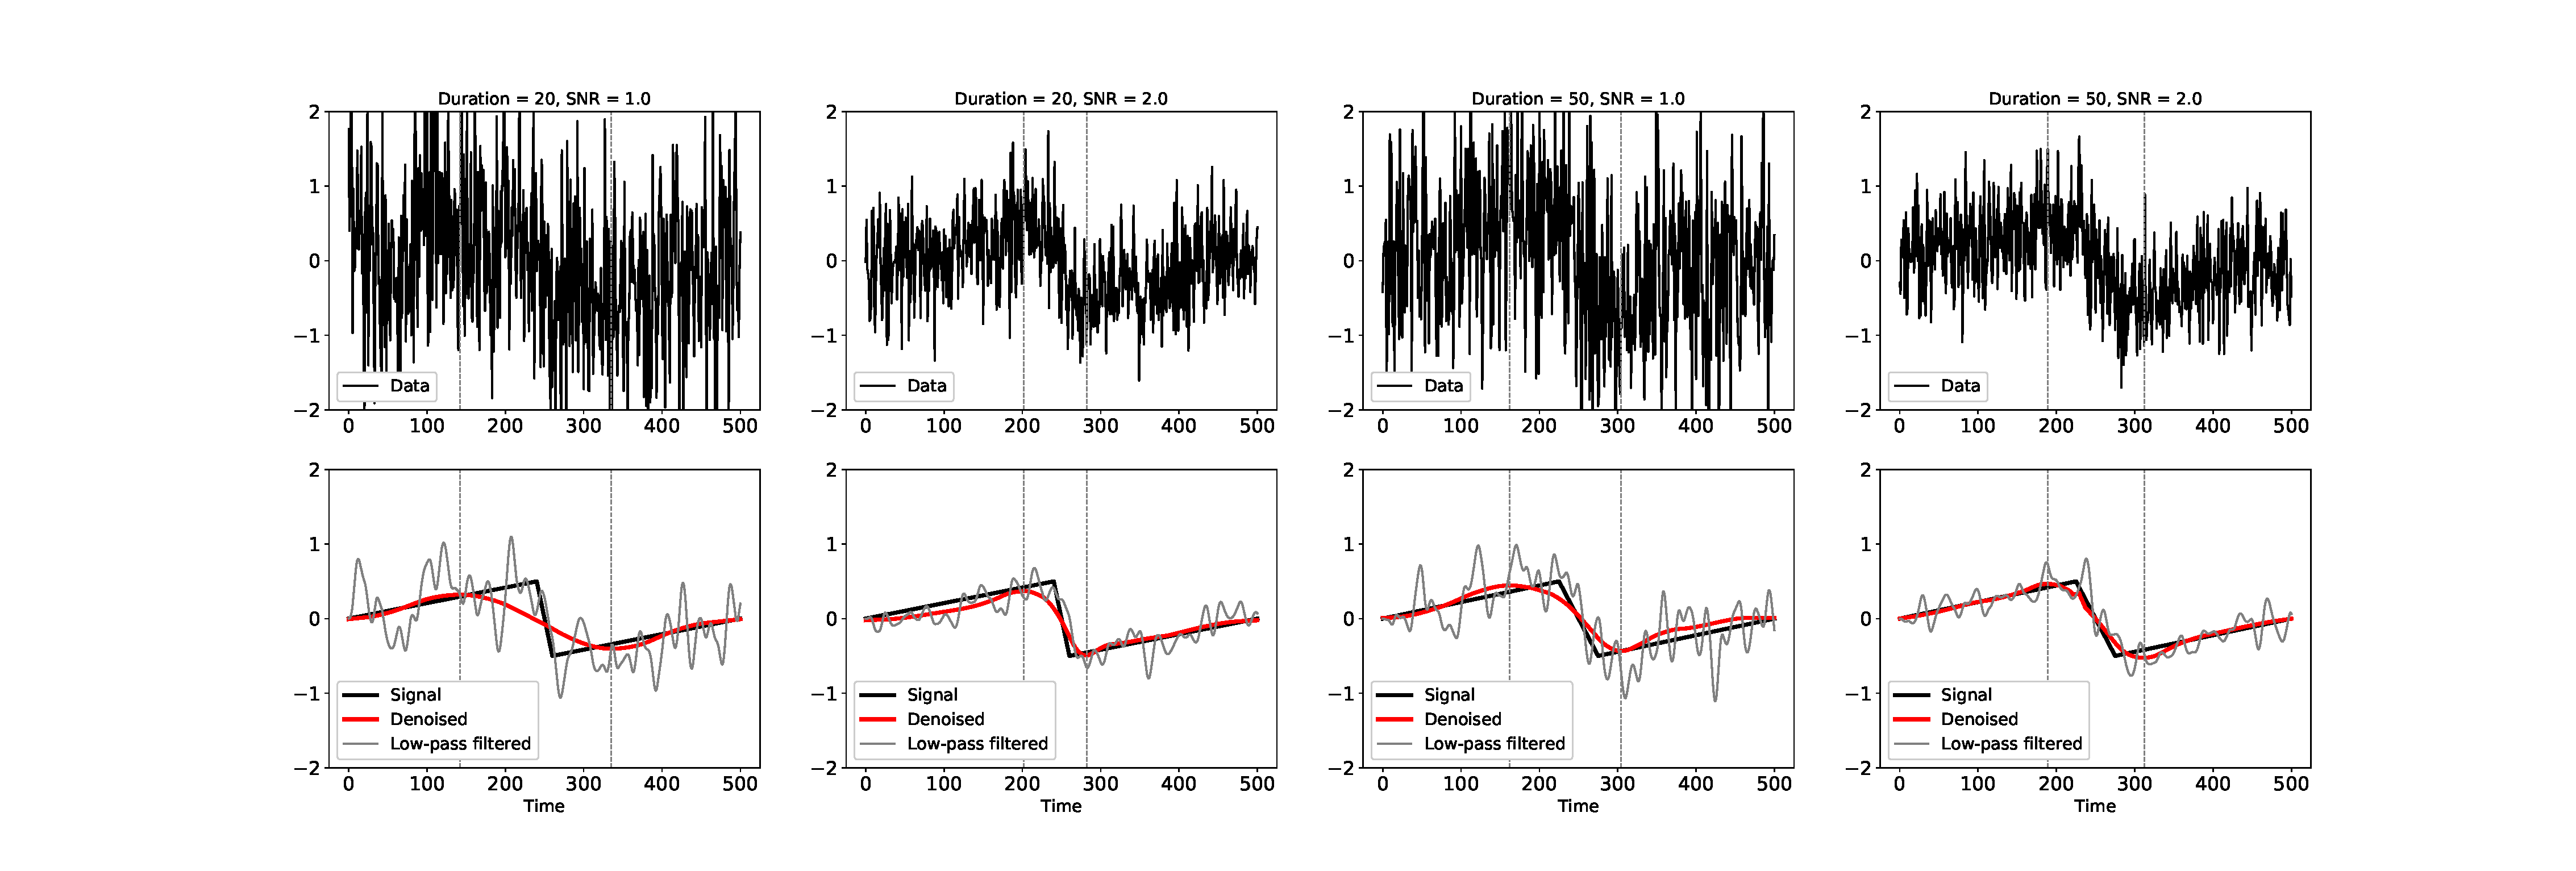
\includegraphics[trim={8.5cm 1cm 7.5cm 2cm}, clip, width=450pt]{figures/slowslip_synthetics.eps}
\captionsetup{type=figure}
\captionof{figure}{Denoising of synthetic time series using wavelets for two durations of the slow slip and two signal-to-noise ratios. The black line on the bottom panels is the signal. The black line on the top panels is the signal to which a Gaussian noise has been added. The red line on the bottom panels is the denoised signal obtained using thresholding of the wavelet vectors. The two vertical dashed lines show the time of the maxima and minima of the denoised signal. The grey line on the bottom panels is the signal obtained with a low-pass filter.}
\end{center}

\begin{center}
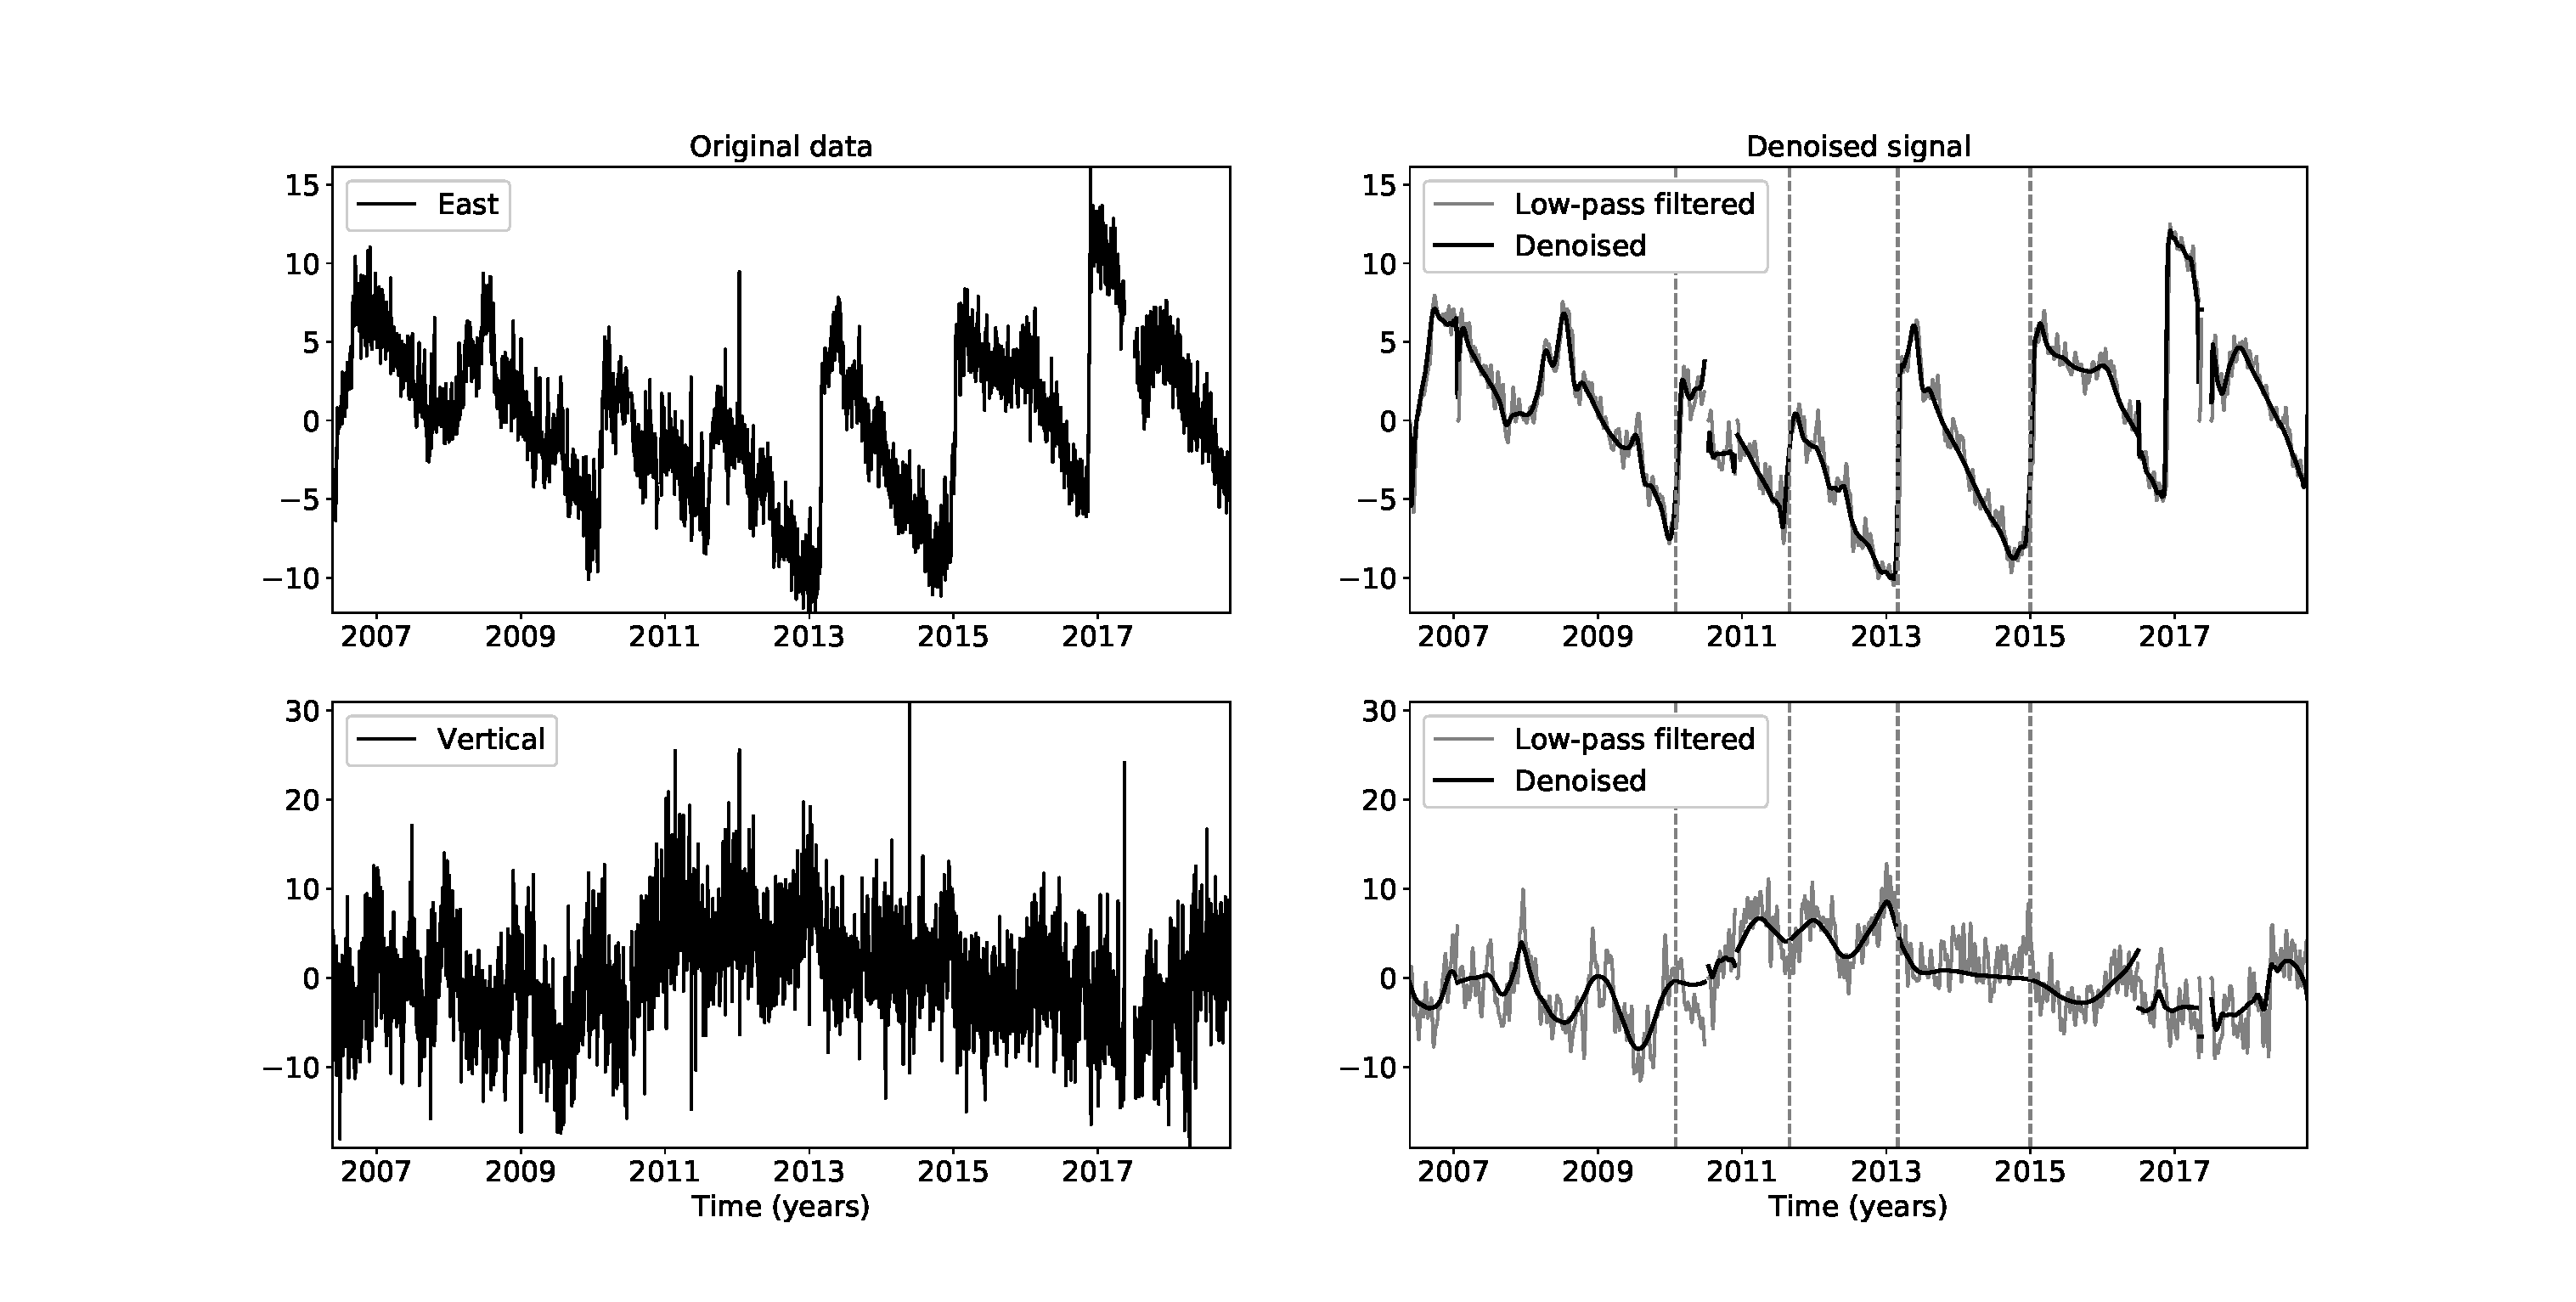
\includegraphics[trim={5cm 1cm 5cm 2cm}, clip, width=450pt]{figures/slowslip_denoising.eps}
\captionsetup{type=figure}
\captionof{figure}{Original (left) and denoised (right) displacement observed at GPS station CKID for the eastern (top) and vertical (bottom) components. The black line on the right panels is the denoised signal obtained using thresholding of the wavelet vectors. The grey line on the right panels is the signal obtained with a low-pass filter. The vertical dashed lines indicate the timing of the slow slip events identified by Todd and Schwartz (2016 ~\cite{TOD_2016}).}
\end{center}

\end{document}
